%----------------------------------------------------------------
%
%  File    :  analyse.tex
%
%  Author  :  Thomas Fragner
% 
%  Created :  2017-10-01
% 
%  Changed :  2018-04-10
% 
%----------------------------------------------------------------

\chapter{Erkennung sequenzieller Legestrukturen} % (fold)
\label{cha:erkennung}
Nachdem in Kapitel \ref{cha:hintergrund} die Grundlage zum Verständnis von sequenziell gelegten Prozessen in CMB Modellen  dargestellt wurde, werden in diesem Kapitel das notwendige Ausgangsmaterial, die Kriterien bzw. die Strategie zur Erkennung dieser Strukturen untersucht. Diese Erkenntnisse bilden die Basis für den Algorithmus.

\section{Allgemeine Einschränkung} % (fold)
\label{sec:allgmeine_einschrankung}
Der zu entwickelnde Algorithmus kann nur Strukturen erkennen, die auch ein Mensch ohne genaue inhaltliche Kenntnisse des Prozesses ableiten kann. Das heißt, dass nur geometrische Anordnungen bei der Erkennung berücksichtigt werden. Diese Anordnungen müssen im weitesten Sinne einen linearen sequenziellen Zusammenhang erkennen lassen.
% section allgmeine_einschrankung (end)

\section{Ausgangsmaterial} % (fold)
\label{sec:ausgangsmeterial}
Der Algorithmus verarbeitet nicht das Basisbildmaterial direkt, sondern verwendet eine bereits digitalisierte Repräsentation die durch den Model Digitizer \cite{opplstary2017}, welcher Bildmaterial in SVG Grafiken umwandelt, erzeugt wird.

Folgende Daten werden vom Model Digitizer pro Karte zur Verfügung gestellt und dienen als Eingangsdaten für den Algorithmus:
\begin{itemize}
	\item eindeutige Karten-ID
	\item Kartentyp
	\begin{itemize}
		\item Subjekt
		\item Aufgabe
		\item Austausch
	\end{itemize}
	\item X- und Y-Koordinaten für die Eckpunkte der Karte. 
\end{itemize}
% section ausgangsmeterial (end)

\section{Problemstellungen} % (fold)
\label{sec:problemstellungen}
Bei der algorithmischen Auswertung sequenzieller Abfolgen ergeben sich 4 Hauptkriterien, welche bei der Interpretation berücksichtigt werden müssen:
\begin{enumerate}
	\item Abweichungen von den Legevorschriften laut CBM.
	\item Ungenaue Positionierung der Karten.
	\item Unterschiedliches Ausgangsbildmaterial.
	\item Fehlerhafte Interpretation durch den Model Digitizer.
\end{enumerate}

\subsection{Abweichungen von den Legevorschriften} % (fold)
\label{ssub:abweichung_von_der_legevorschriften}
Basierend auf den Testbeispielen \cite{max} ergeben sich Abweichungen, die eine algorithmische Verarbeitung der Daten unmöglich machen oder erschweren.

Aus den Testbeispielen haben sich zwei grundsätzliche Legemuster ergeben:

\begin{itemize}
	\item Linienlayout (siehe Abbildung ~\ref{fig:linienlegemethode}) 
	\item Sternlayout (siehe Abbildung ~\ref{fig:sternlegemethode}) 
\end{itemize}

\begin{figure}[h]
	\centering 
	\begin{minipage}[b]{0.45\textwidth} 
		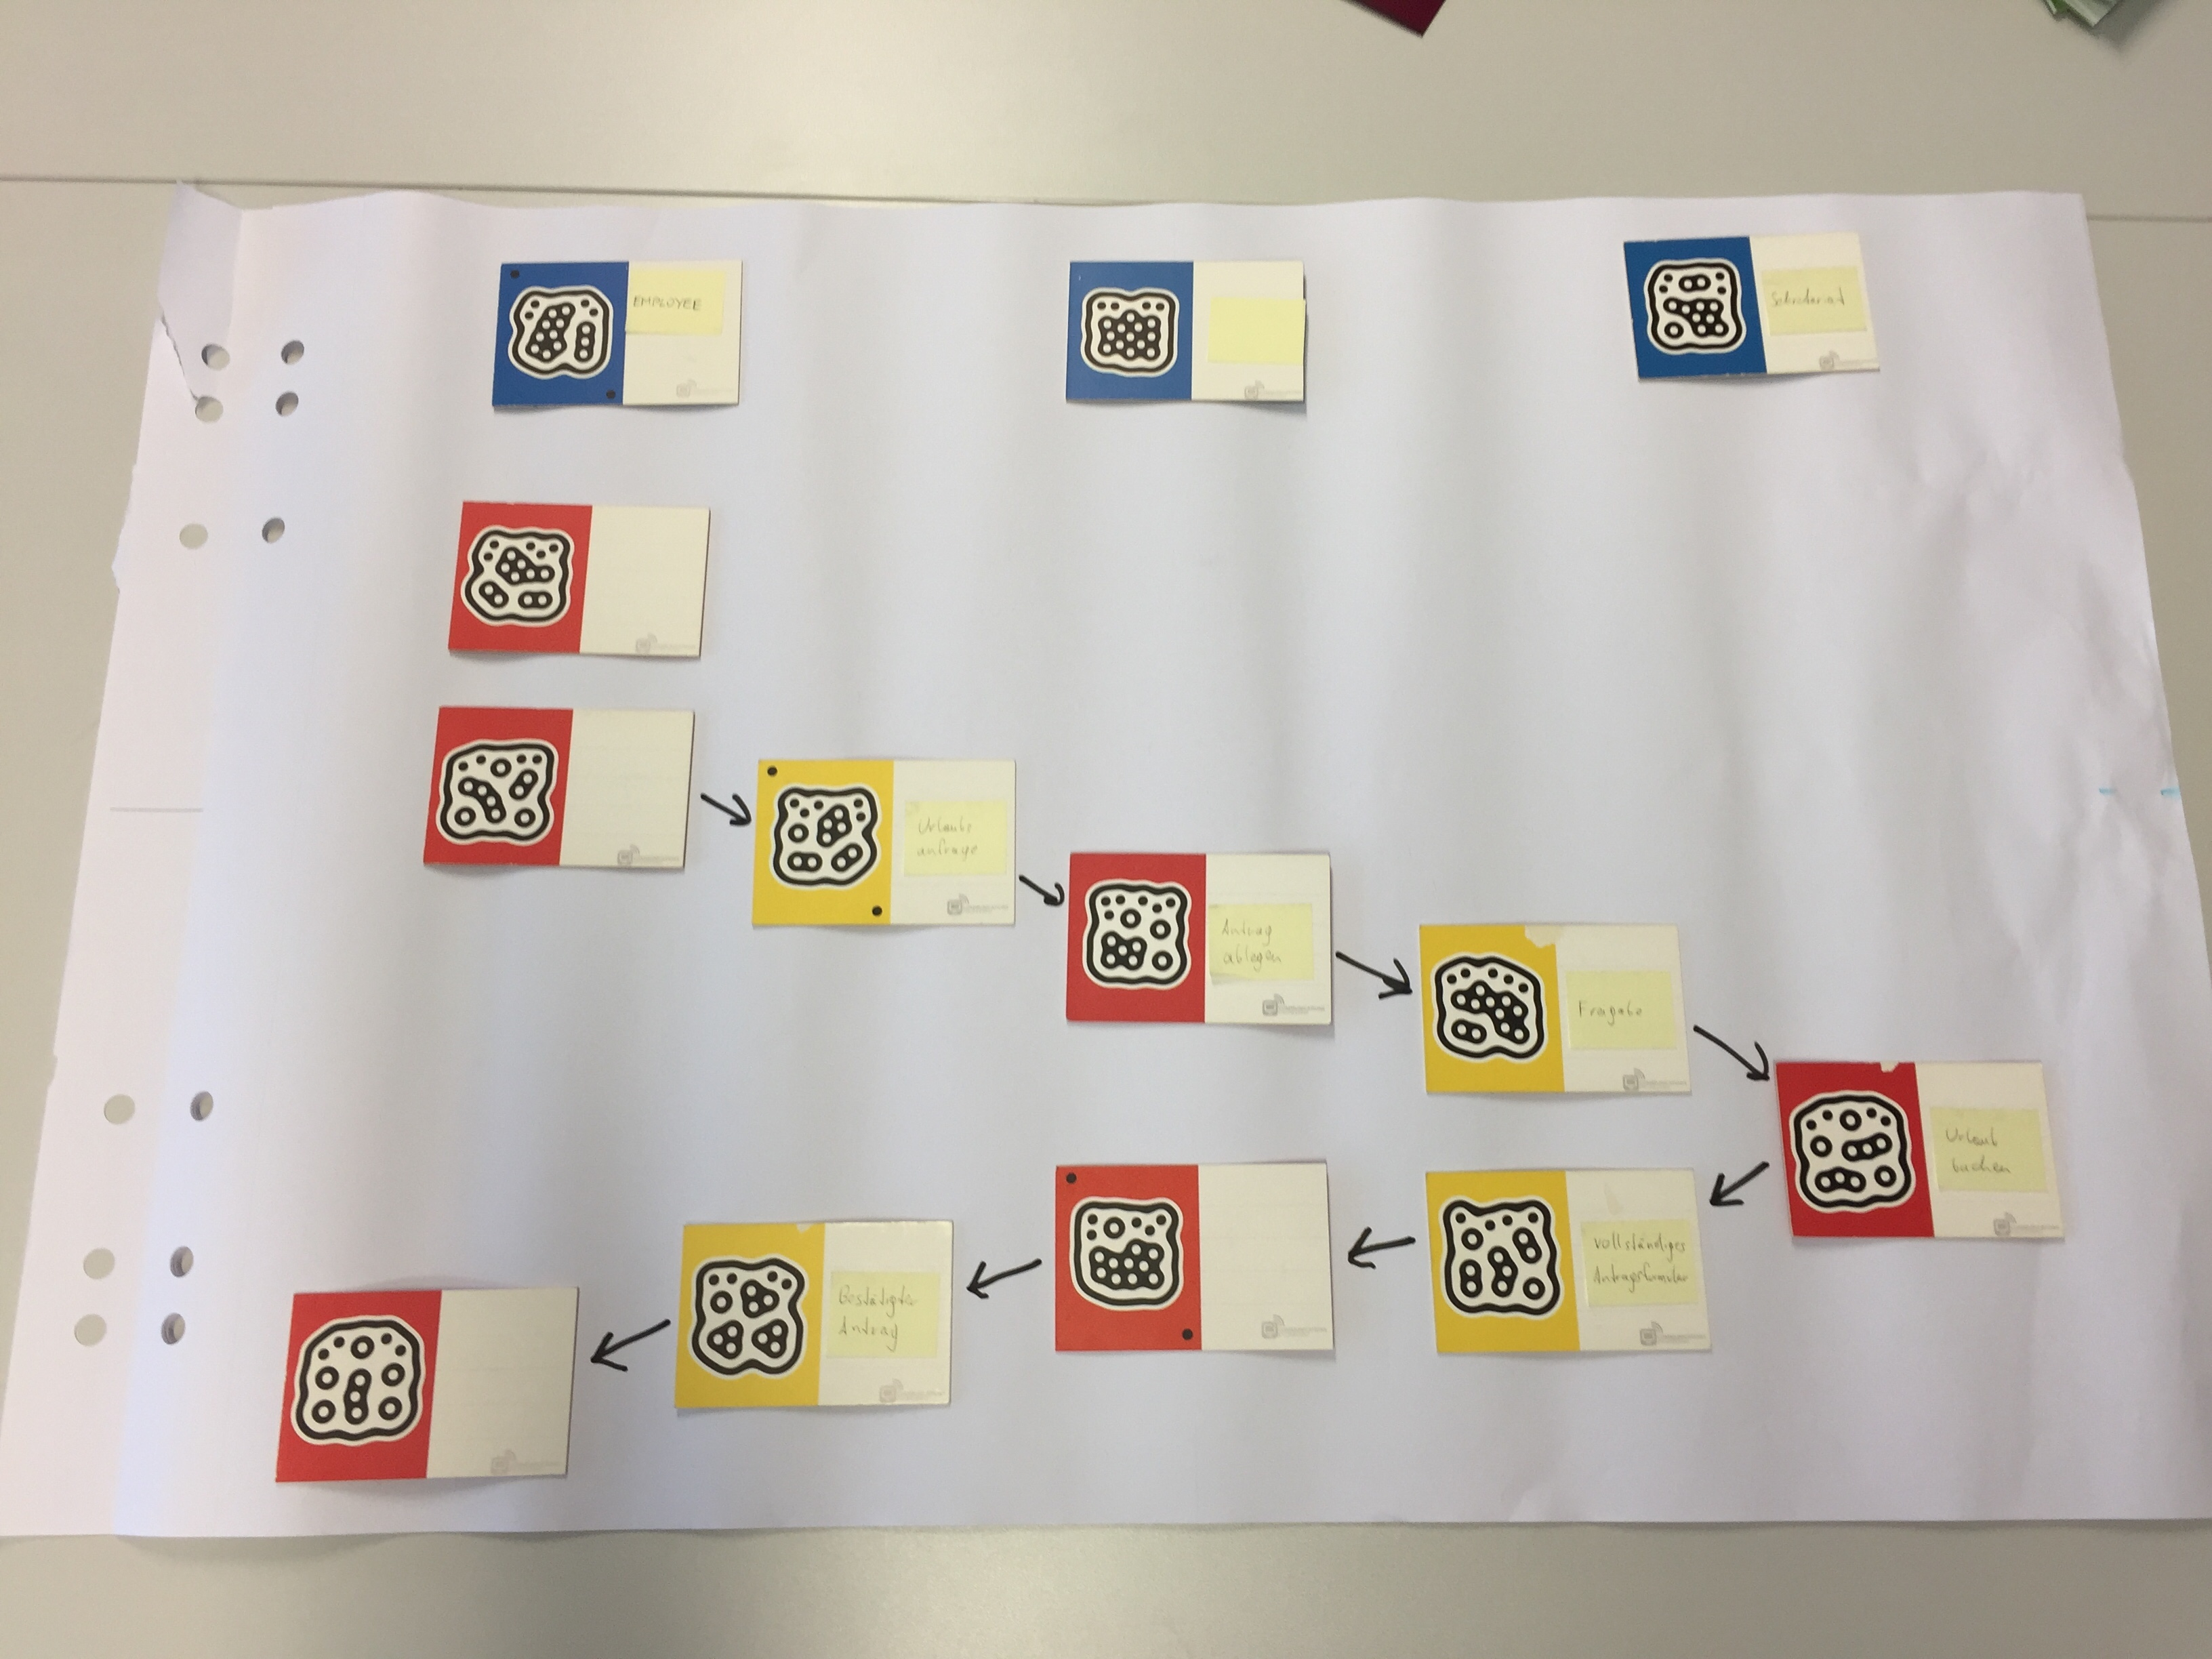
\includegraphics[width=\textwidth]{figures/linienlegemethode.jpg}
		\caption[Linienlayout]{Linienlayout  \protect~\cite{max}}
		\label{fig:linienlegemethode} 
	\end{minipage}
	\hfill 
	\begin{minipage}[b]{0.45\textwidth} 
		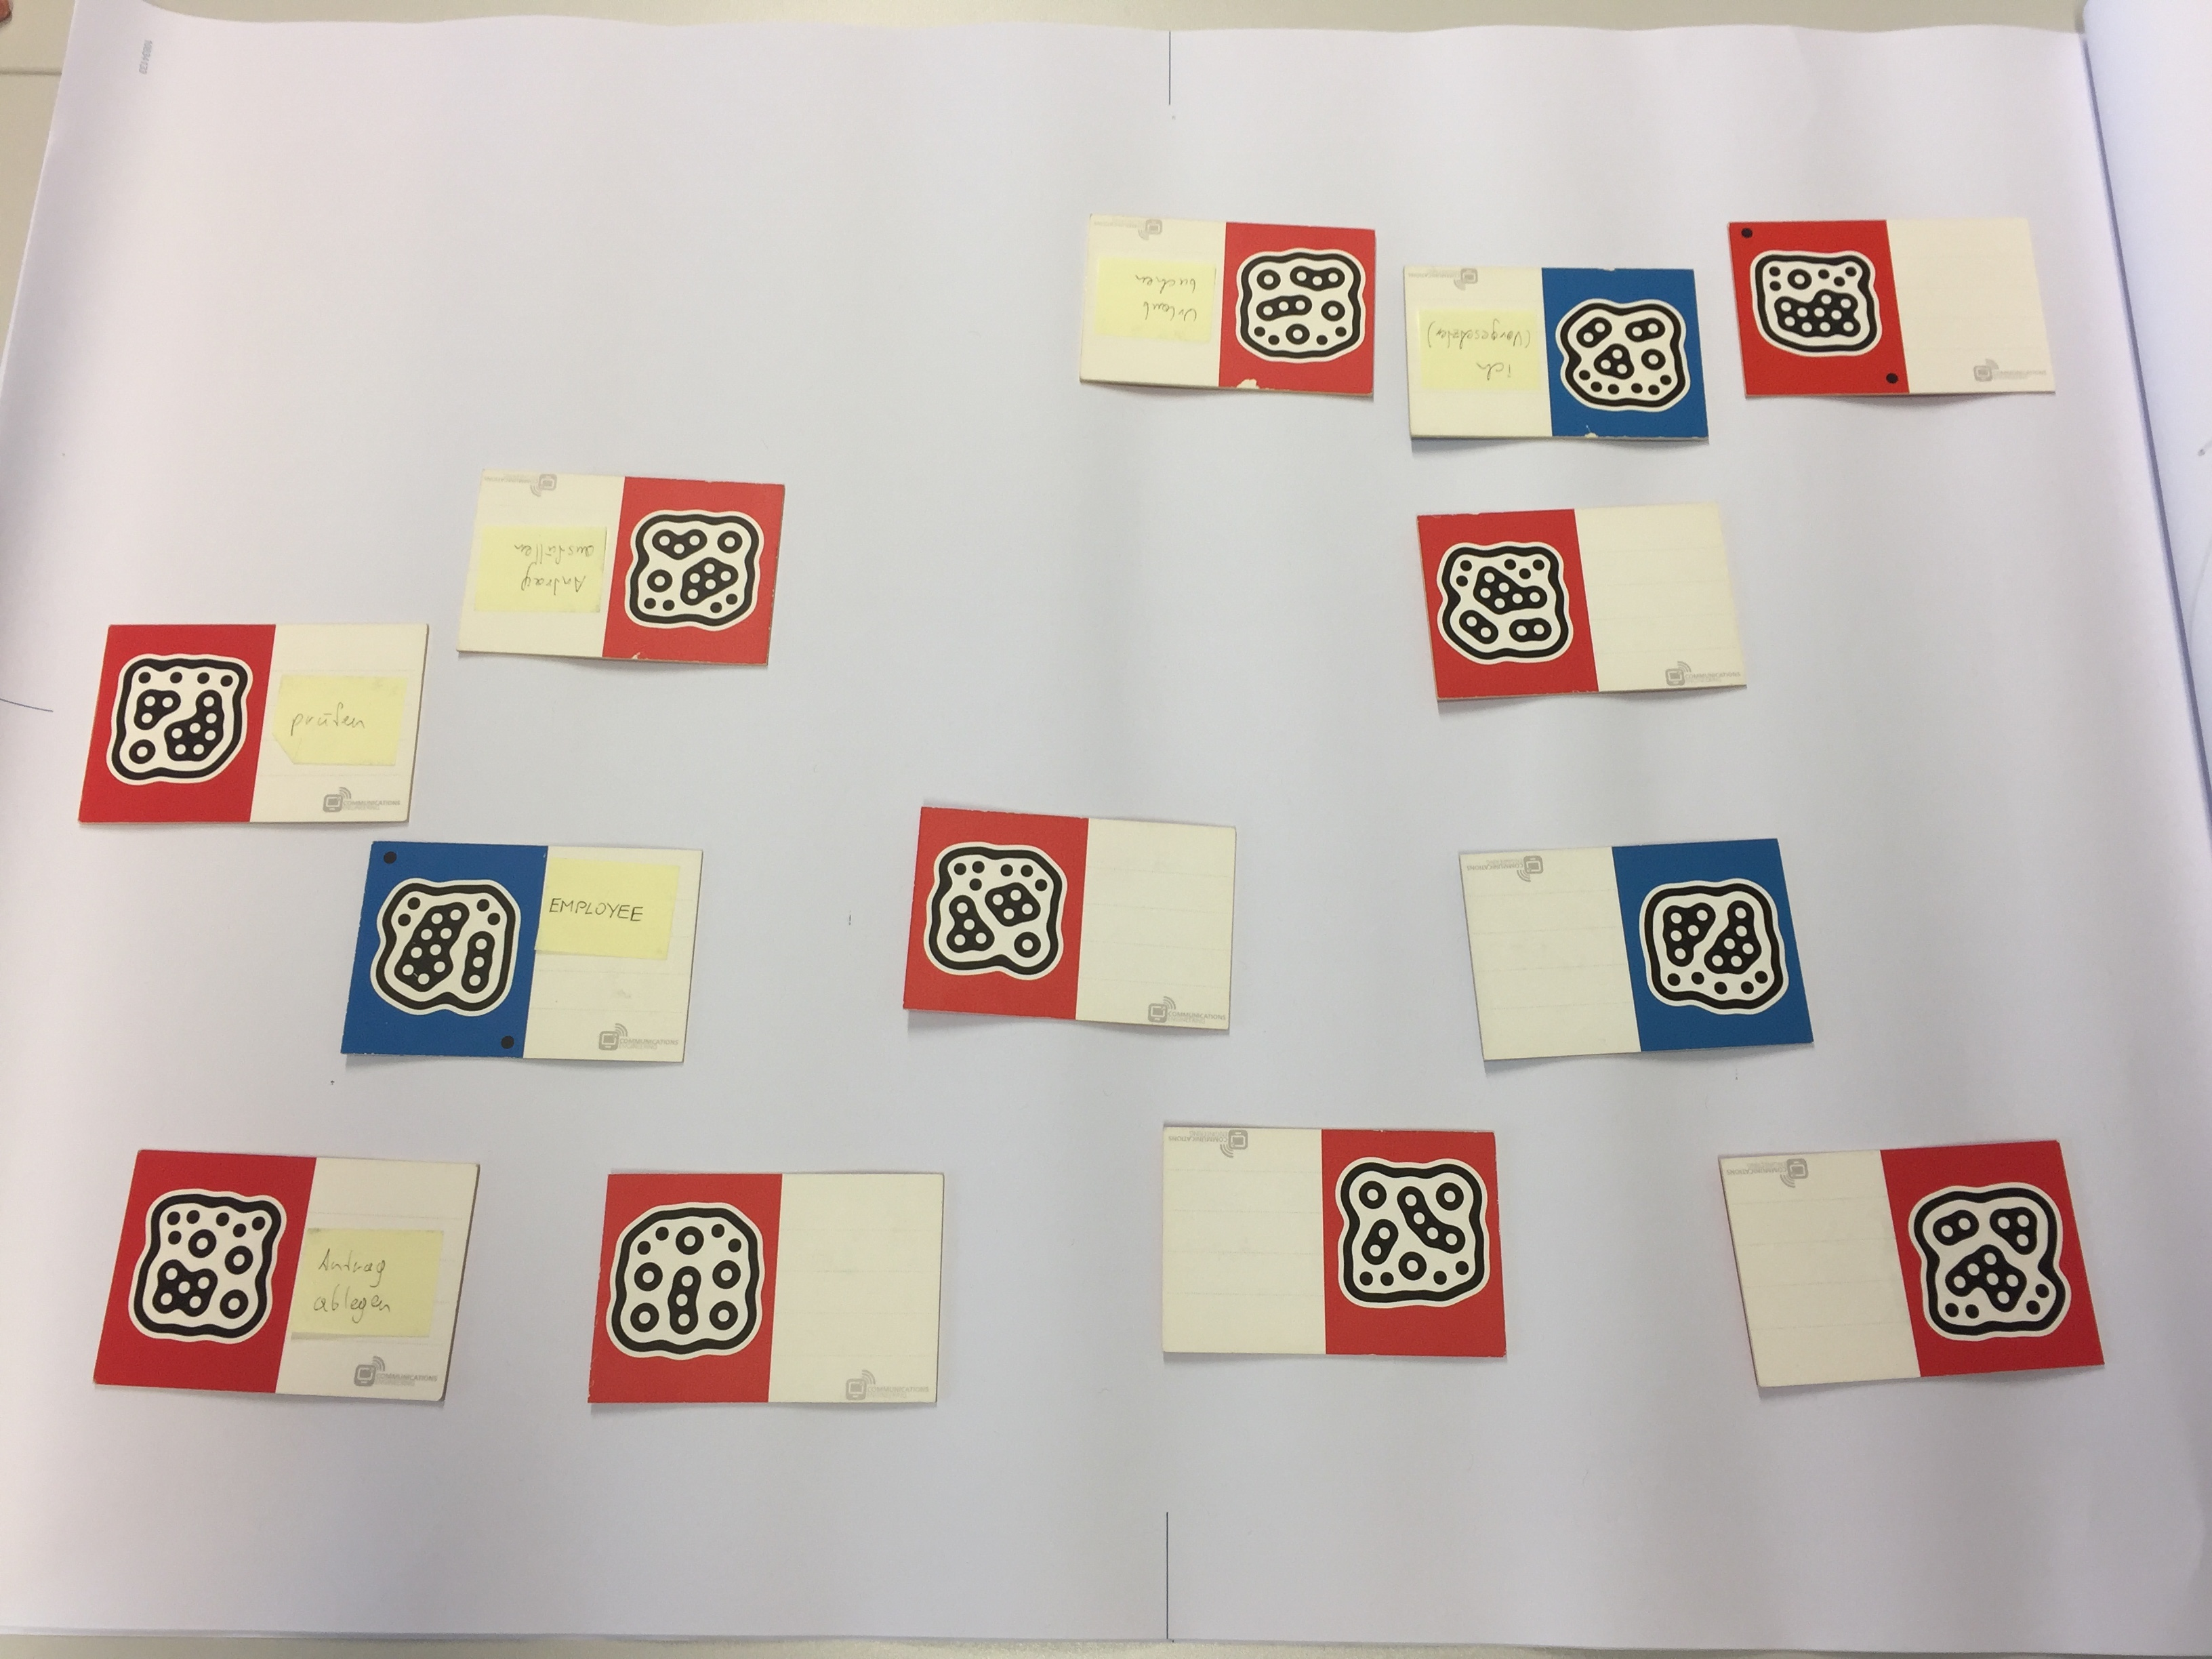
\includegraphics[width=\textwidth]{figures/sternlegemethode.jpg}
		\caption[Sternlayout]{Sternlayout \protect~\cite{max}}
		\label{fig:sternlegemethode} 
	\end{minipage}
\end{figure}

Das Linienlayout entspricht den vorgegebenen Legevorschriften. Beim Sternlayout werden die Vorschriften nicht beachtet. Es ergeben sich daraus folgende Problemstellungen:
\begin{itemize}
	\item Es kann kein Startelement erkannt werden, da alle Aufgaben annähernd gleich weit vom nächstgelegenem Subjekt entfernt sind.
	\item Es ist keine sequenzielle Struktur ausgehend vom Subjekt erkennbar, und daher kann kein chronologischer Zusammenhang zwischen den Aufgaben abgeleitet werden.
\end{itemize}

Aufgrund dieser Merkmale ist das Sternlayout nicht zur Analyse geeignet, aber es ergibt sich die Anforderung diese beiden Layouttypen voneinander unterscheiden zu können.

Weitere Abweichungen betreffen die Anordnung der Subjekte und die Legerichtung der Aufgaben. In Abbildung \ref{fig:subjekt-position} sind die Subjekte entgegen den Vorschriften nicht horizontal auf einer Linie am oberen Bildrand angeordnet. Abbildung \ref{fig:nicht-vertikal} zeigt, dass die Aufgaben nicht vertikal ausgehend vom Subjekt angeordnet sind.

Obwohl die Legevorschriften bei beiden Prozessmodellen nicht eingehalten werden, sind die chronologischen Subjekt/Aufgabe Zuordnungen klar ersichtlich. Diese Muster sollten vom Algorithmus daher richtig erkannt werden. 

\begin{figure}[h]
	\centering 
	\begin{minipage}[b]{0.45\textwidth} 
		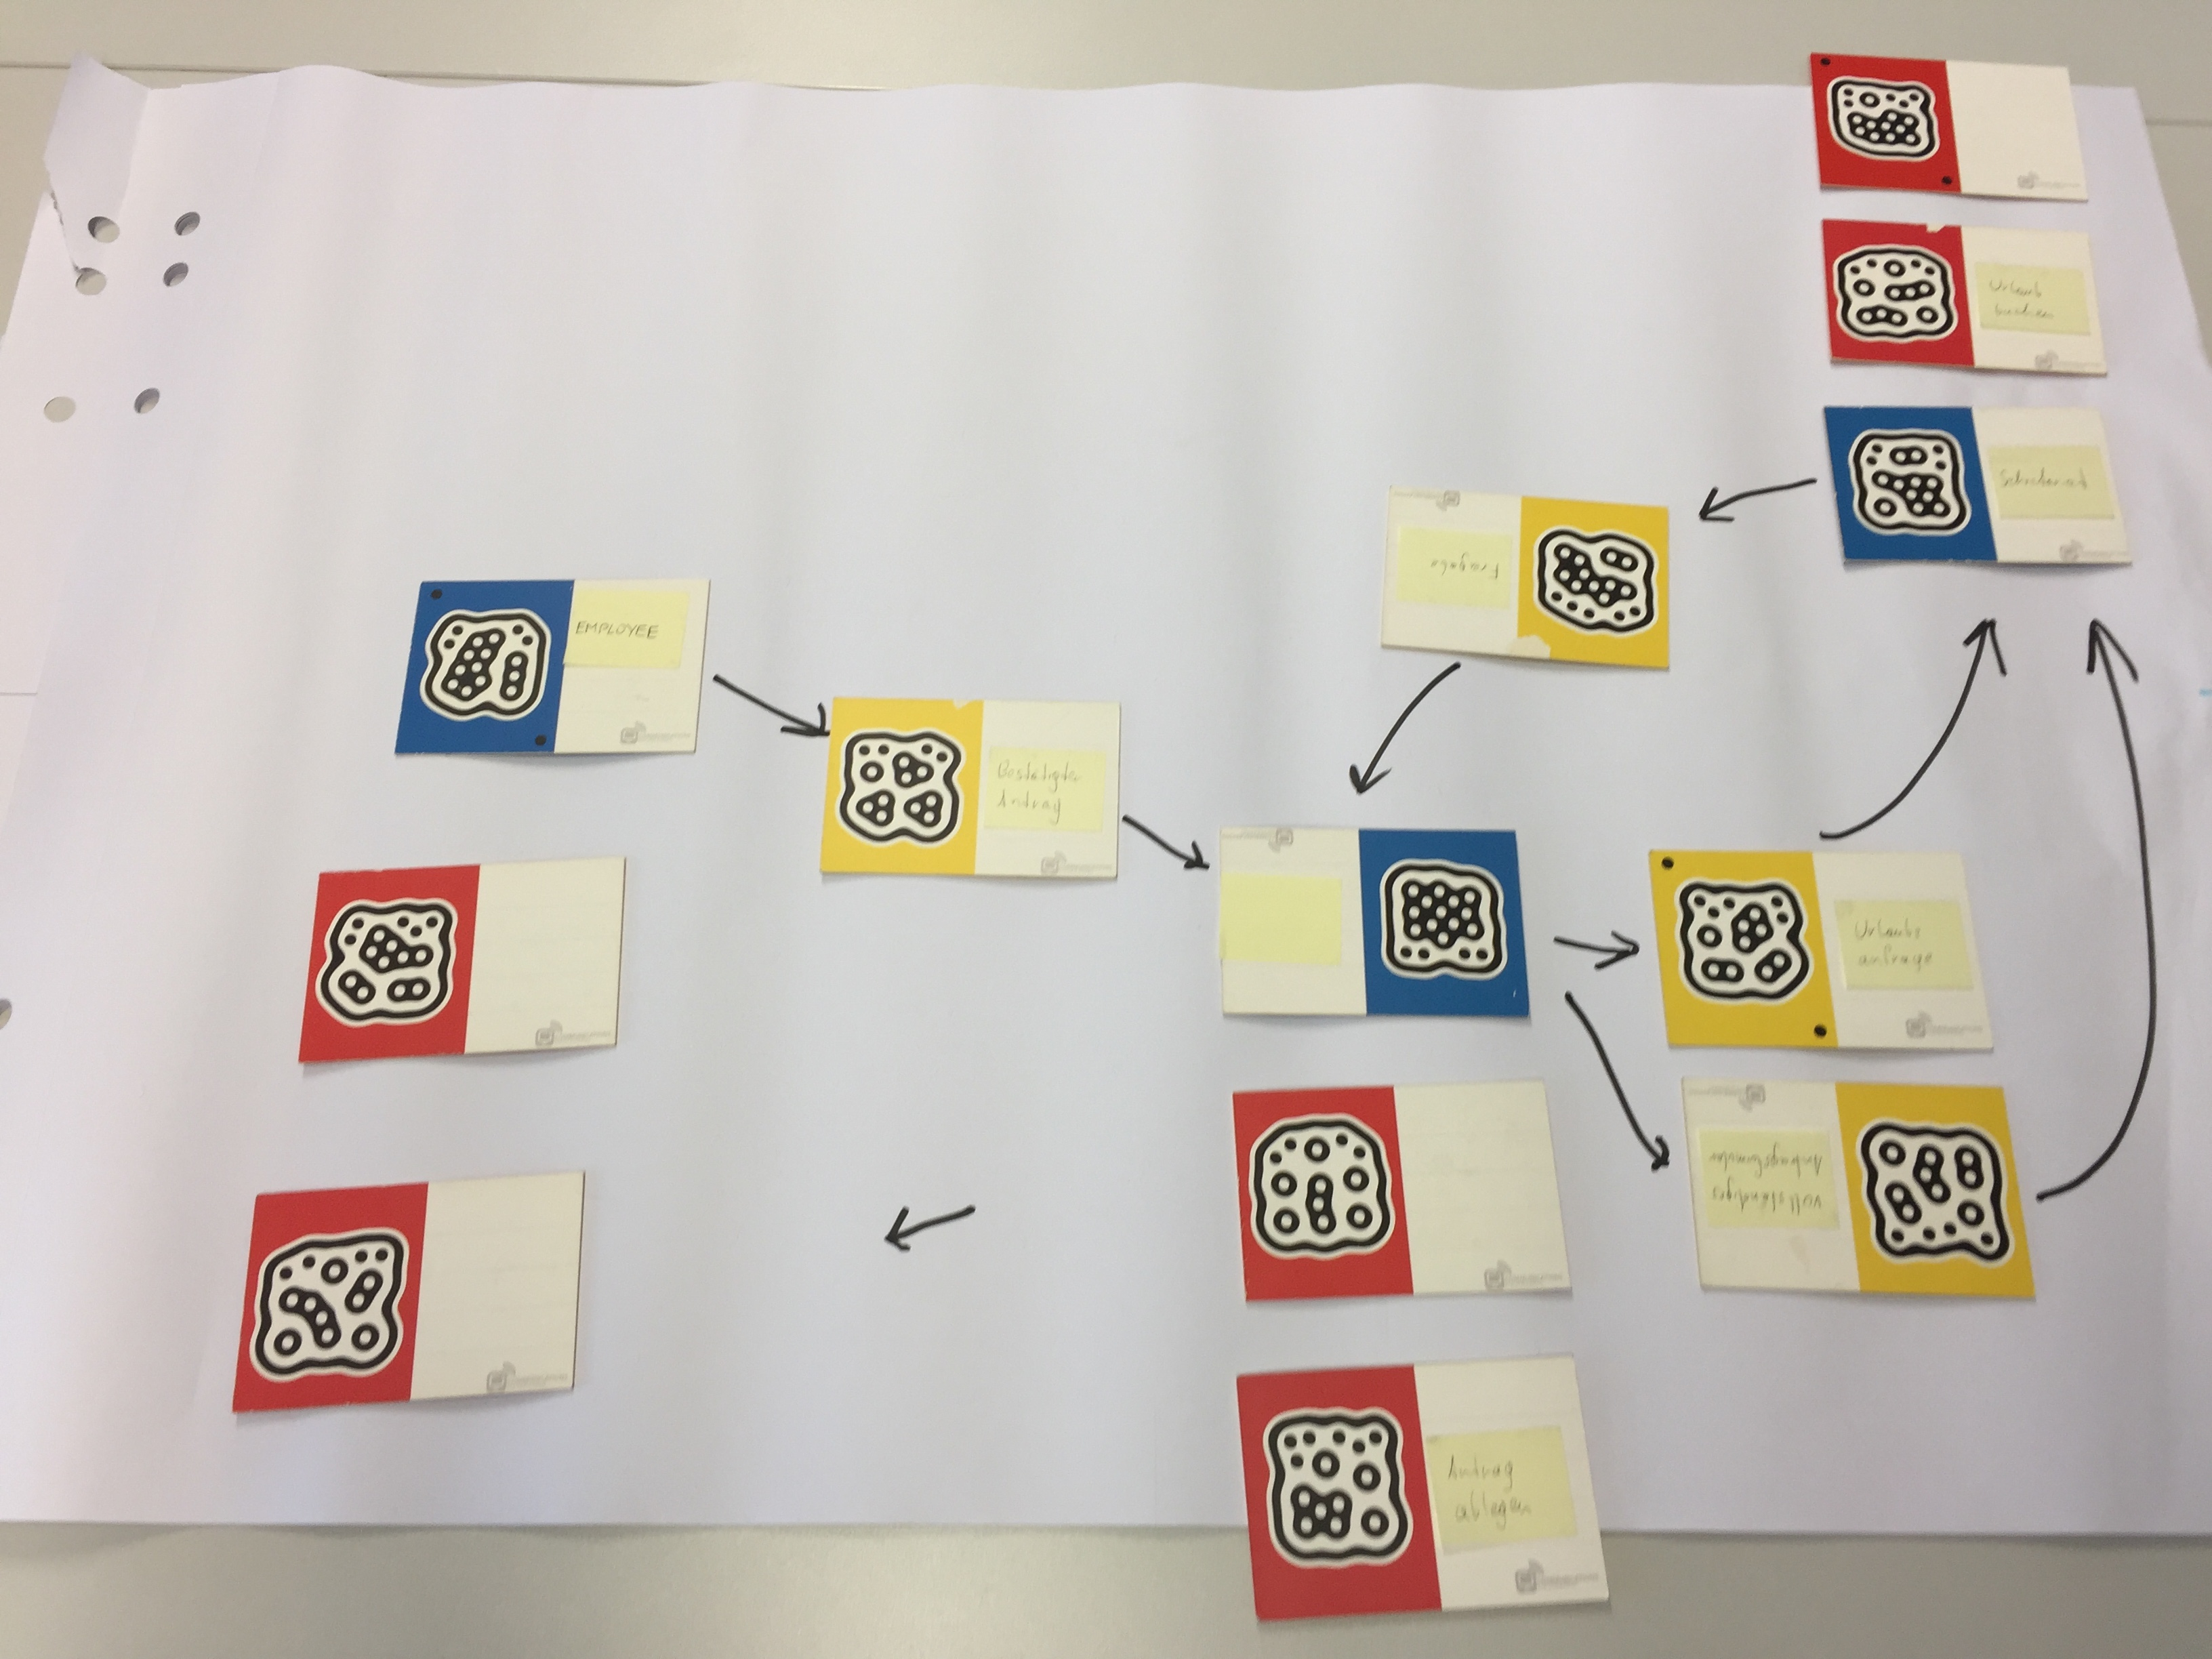
\includegraphics[width=\textwidth]{figures/03.jpg}
		\caption[Subjektposition]{Subjektposition \protect~\cite{max}}
		\label{fig:subjekt-position} 
	\end{minipage}
	\hfill 
	\begin{minipage}[b]{0.45\textwidth} 
		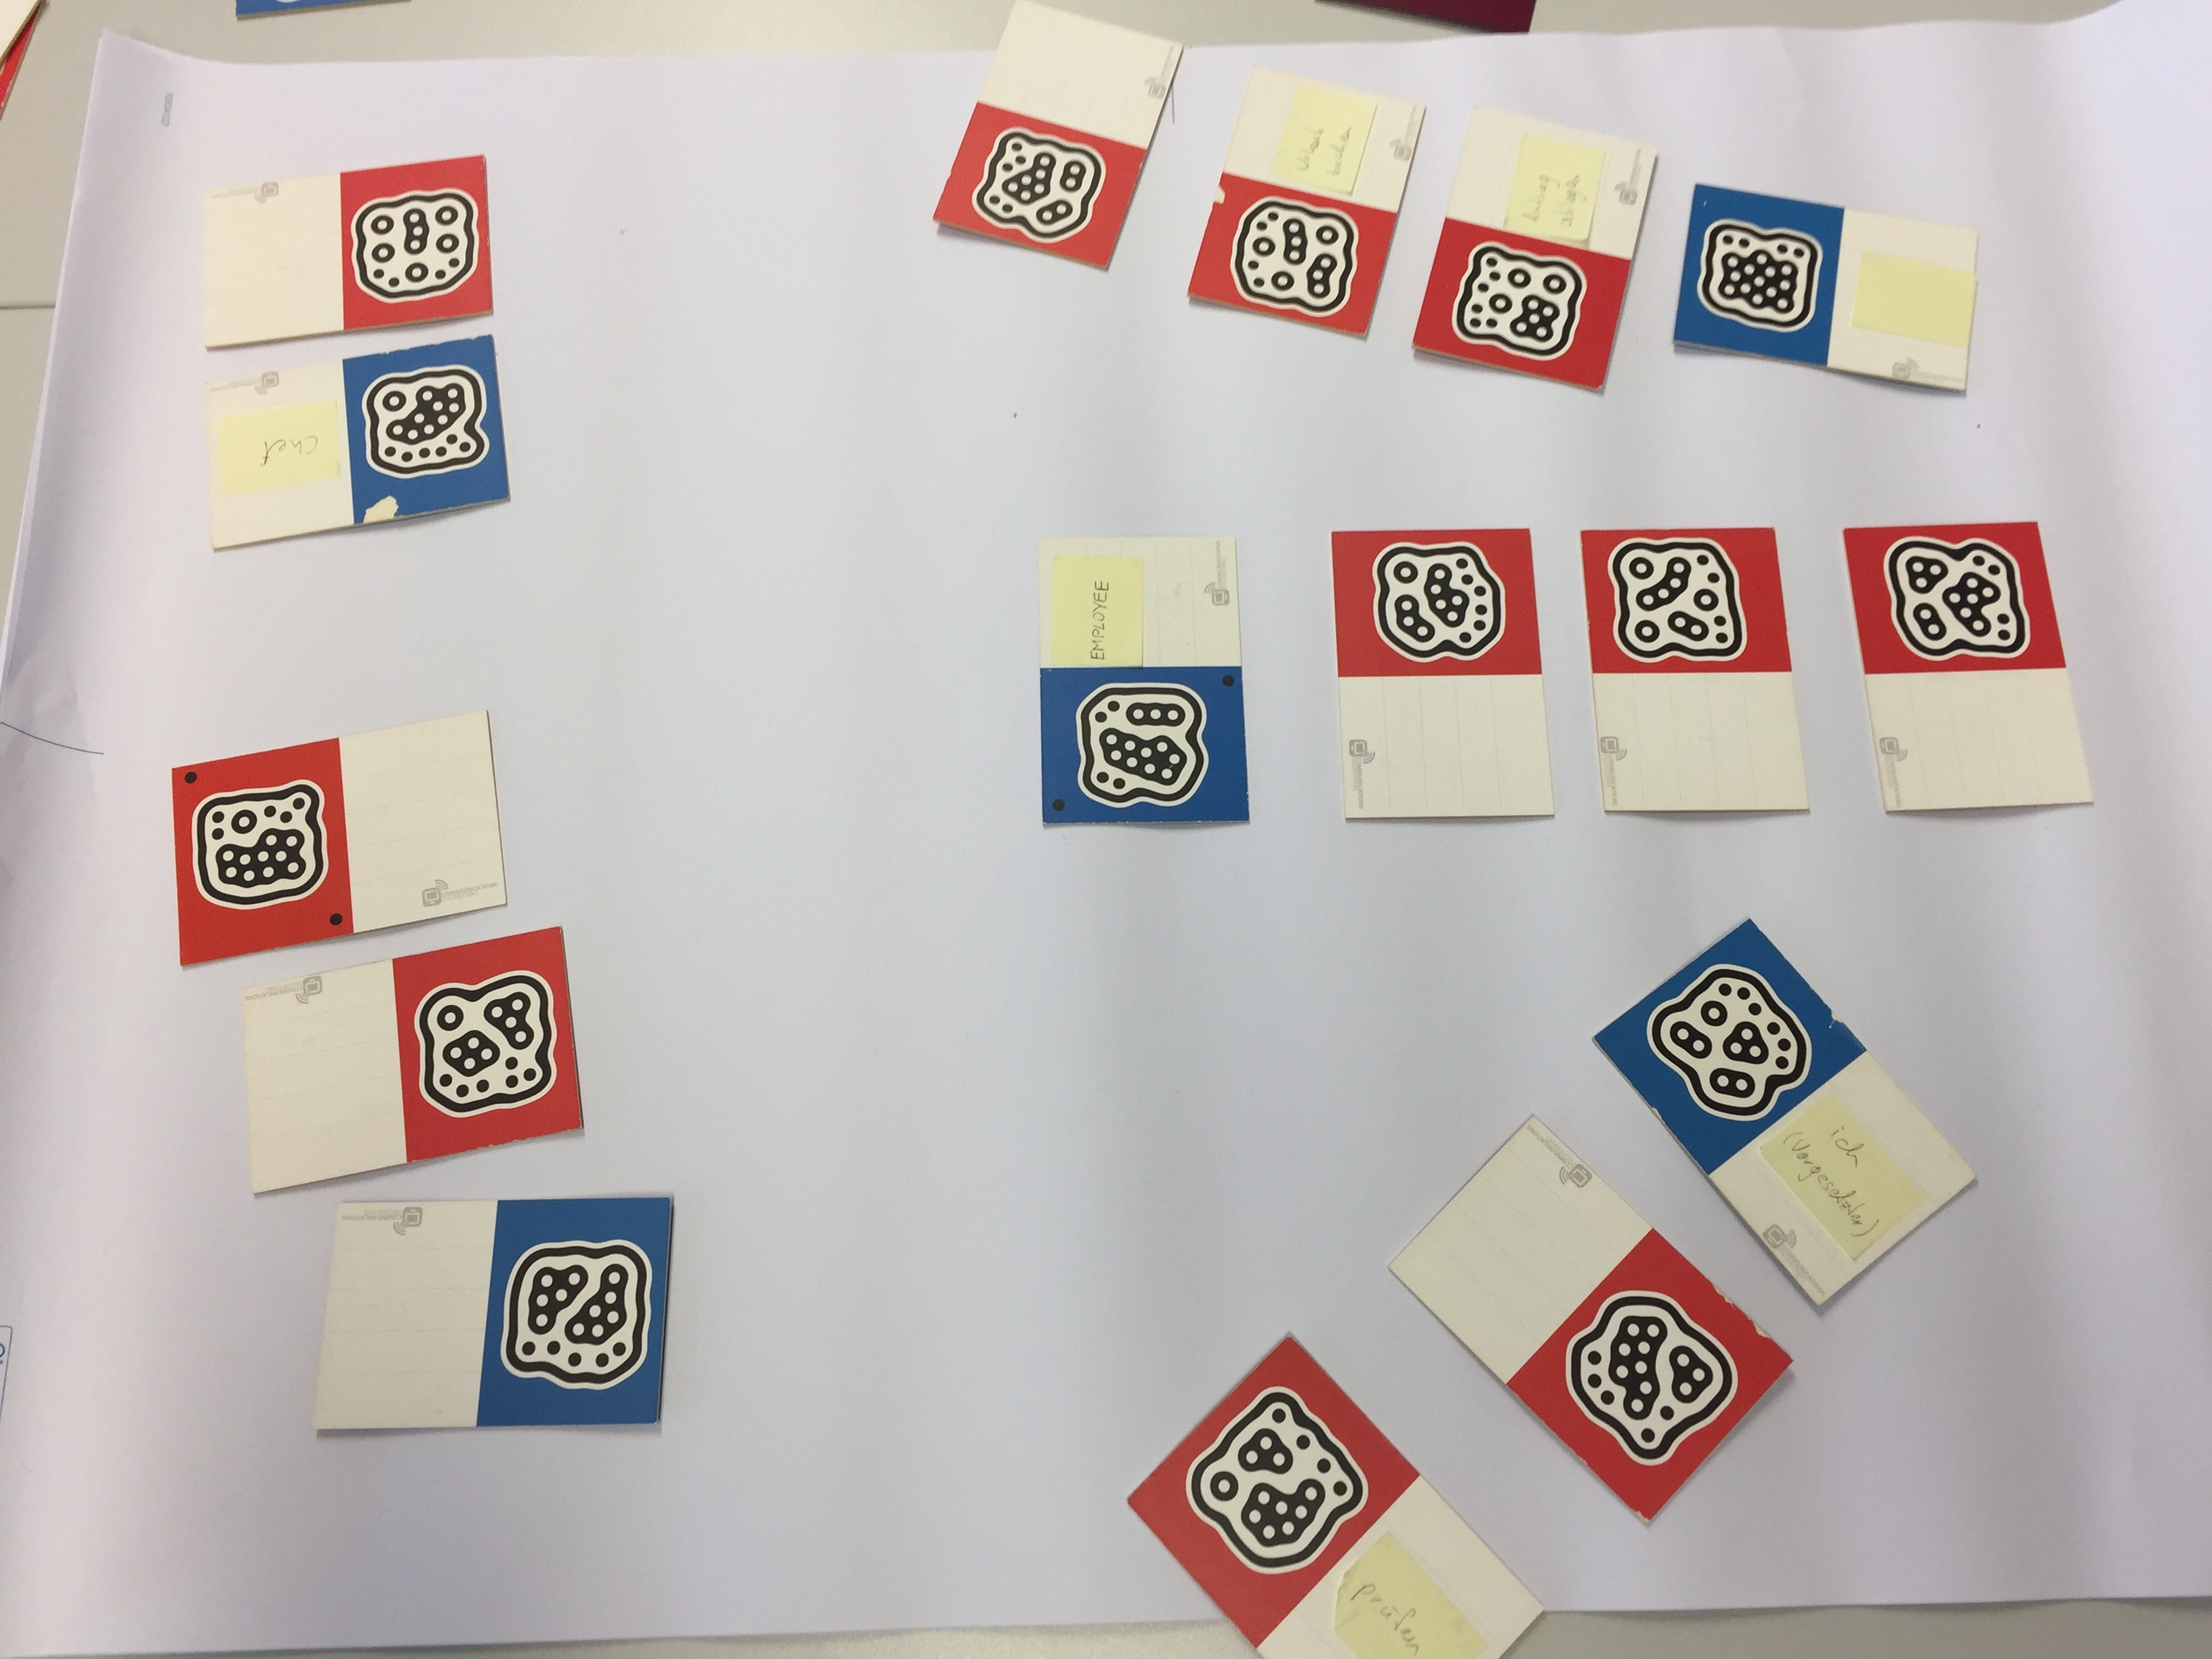
\includegraphics[width=\textwidth]{figures/17.jpg} 		
		\caption[Richtungsunterschiede]{Richtungsunterschiede \protect~\cite{max}}
		\label{fig:nicht-vertikal} 
	\end{minipage}
\end{figure}
% subsubsection abweichung_von_der_legevorschrift (end)

\subsection{Ungenaue Kartenlegung} % (fold)
\label{ssub:ungenaue_kartenlegung}
Mit der Methode des Kartenlegens verbunden, ist die ungenaue Positionierung und Lage der Karten. In Abbildung \ref{fig:karten-position} ist ersichtlich, dass die roten Aufgabenkarten nicht exakt unterhalb des Subjekts angeordnet sind und auch eine Rotation dieser Karten feststellbar ist. Diese Ungenauigkeiten sollten vom Algorithmus innerhalb einer bestimmten Toleranz ebenfalls richtig interpretiert werden.

\begin{figure}[h]
	\centering 
	\begin{minipage}[b]{0.8\textwidth} 
		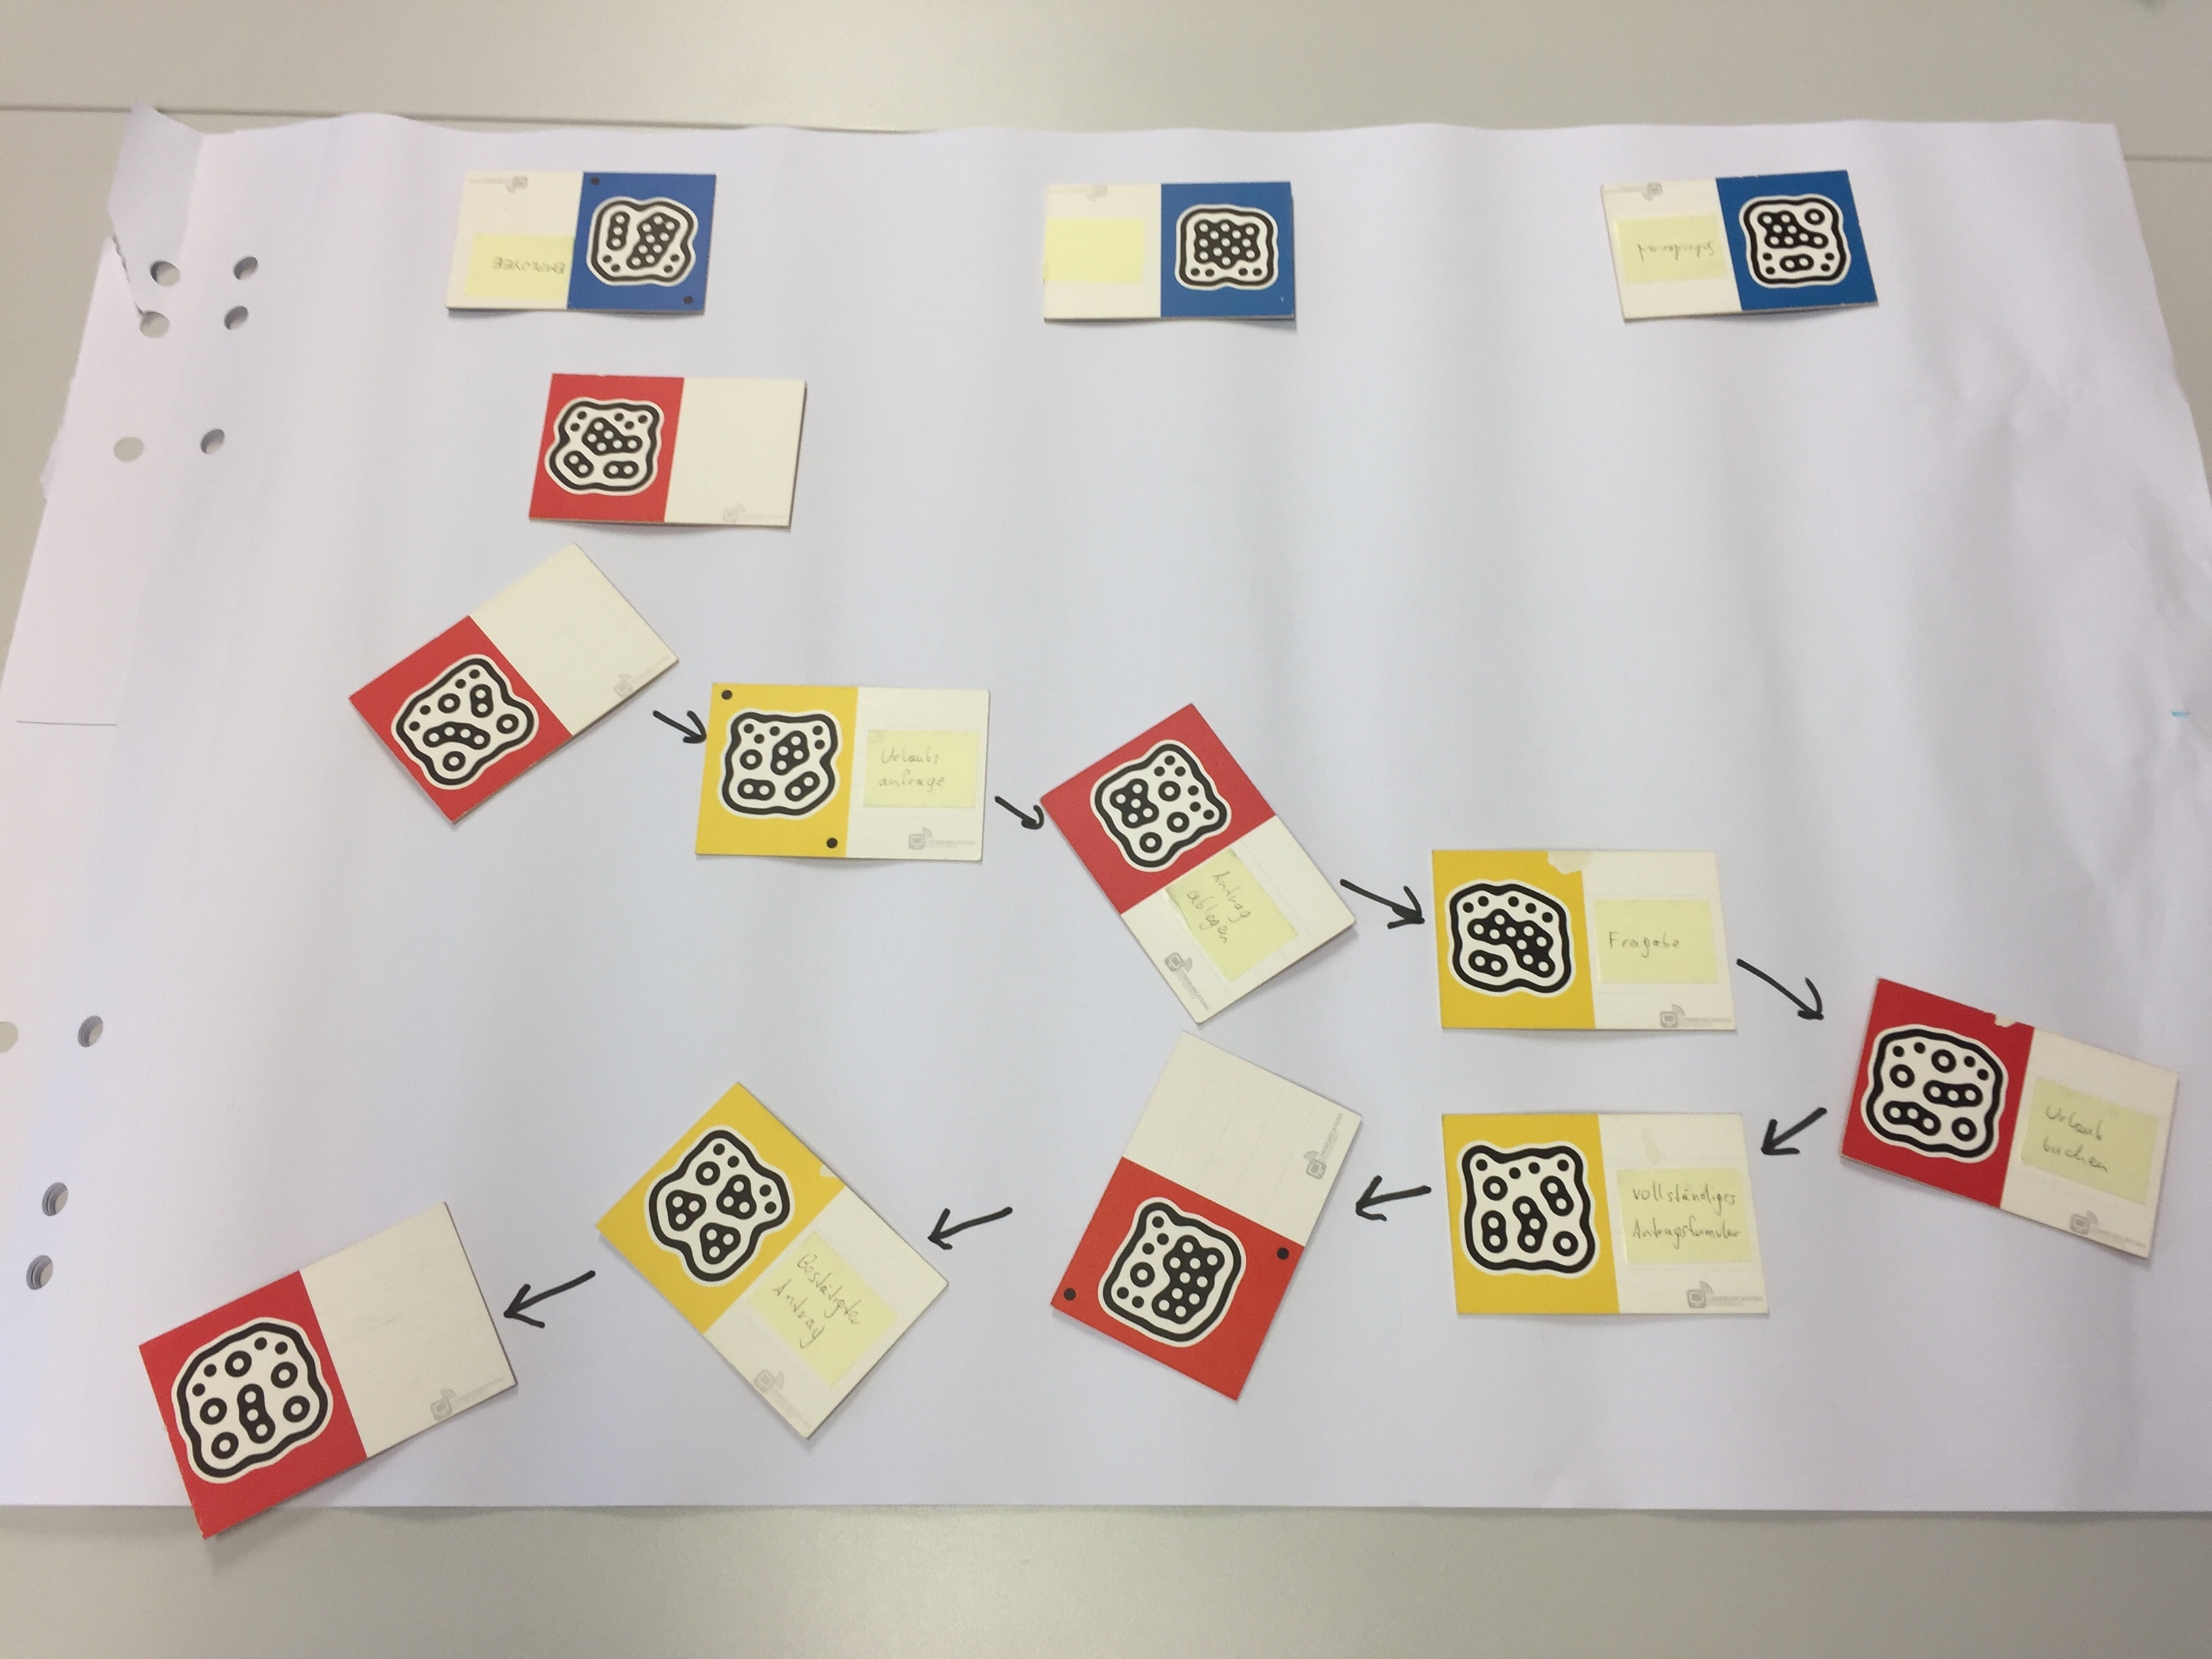
\includegraphics[width=\textwidth]{figures/02.jpg}
		\caption[Kartenposition und -orientierung]{Kartenposition und -orientierung  \protect~\cite{max}}
		\label{fig:karten-position} 
	\end{minipage}
\end{figure}
% subsubsection ungenaue_kartenlegung (end)

\subsection{Ausgangsbildmaterial} % (fold)
\label{sub:ausgangsbildmaterial}
Im ersten Schritt der Digitalisierung wird mit Hilfe von digitalen Aufnahmegeräten ein Bild des Prozesses erstellt. Daraus ergeben sich mehrere Unterschiede im Ausgangsmaterial die potentiell Einfluss auf die algorithmische Auswertung haben:

\begin{itemize}
	\item Auflösung des Bildmaterials
	\item Perspektive der Aufnahme
	\item Bildqualität
\end{itemize}

Die Bildqualität verschlechtert das Ergebnis der Umwandlung in Vektorgrafiken mit Hilfe des Model Digitizer, und beeinflusst somit indirekt den Algorithmus. Die Auflösung bzw. Perspektive wirkt sich auf die Größe der Elemente aus und hat direkten Einfluss auf den Algorithmus. Daher soll der Algorithmus grundsätzlich mit unterschiedlichen Bildmaterialien umgehen können.
% subsection ausgangsbildmaterial (end)

\subsection{Fehlerhafte Basisdaten} % (fold)
\label{sub:fehlerhafte_basisdaten}
Für die Erkennung der sequenziellen Strukturen wird auf eine bereits digitalisierte Version der Rohdaten zugegriffen. Daraus ergibt sich, dass eventuelle Fehler im ersten Digitalisierungsschritt Auswirkungen auf den Algorithmus haben. In den folgenden Kapiteln wird davon ausgegangen, dass die vorhandenen Daten vollständig und richtig sind.
% subsection fehlerhafte_basisdaten (end)
% section problemstellungen (end)

%Die Bilddaten müssen bereits in digitalisierter Struktur vorhanden sein. Dazu kann Bilderkennung und daraus abgleitet eine Vektorgrafik verwendet werden. Diese Vektorgrafik muss im Fall von CBM mindestens die folgenden Grunddaten enhalten.

\section{Erkennungsstrategie} % (fold)
\label{sec:erkennungsstrategie}
Aus den gewonnenen Erkenntnissen (siehe Kapitel \ref{sec:problemstellungen}) und dem bestehenden Algorithmus \cite{max} wird eine grundlegende Strategie zur Erkennung von sequenziell gelegten Prozessen vorgestellt, die als Basis für den Algorithmus dient.

\subsection{Bestehender Algorithmus} % (fold)
\label{sub:unterscheidung_der_legemethode}

% subsection unterscheidung_der_legemethode (end)
\citet{max} schlägt für die Erkennung der Abhängigkeiten die folgenden Algorithmusbestandteile vor:
\begin{description}
	\item[Euklidischer Abstand] Die Aufgaben werden dem Subjekt zugeordnet, zu dem die Aufgabe den geringsten Abstand aufweist.
	\item[Klassifizierung über Quadranten] Für jedes Subjekt werden Quadranten gebildet, und die Aufgaben werden dem Subjekt zugeordnet in dessen Quadrant die Aufgabe liegt.
	\item[Kombination] Die beiden zuvor genannten Methoden werden kombiniert betrachtet um mögliche Falschzuweisungen zu ermitteln.
	\item[Chronologische Ordnung] der Aufgaben wird durch die Abstände zum Subjekt bestimmt.
\end{description}

Zur Verbesserung der Erkennungsgenauigkeit sind weitere Kriterien bzw. Annahmen für die Zuweisungsbestimmung notwendig und werden in den folgenden Kapiteln beschrieben.

\subsection{Anfangselement} % (fold)
\label{sub:anfangselement}
Als Einstiegspunkt für den Algorithmus muss eine Subjekt/Aufgabe Kombination ermittelt werden. Die Kombination mit dem geringsten Abstand zwischen Subjekt und Aufgabe ist der wahrscheinlichste Start des Prozesses und somit der beste Ausgangspunkt um die weiteren Abhängigkeiten zu bestimmen.
\subsection{Richtungsbestimmung} % (fold)
\label{sub:richtungsbestimmung}
Bei einer sequenziell gelegten Anordnung ist eine annähernd gleiche Richtung der Aufgaben zu ihrem Startelement eine Bedingung. Diese Bedingung wurde beim bisherigen Ansatz nur teilweise bei der Klassifizierung nach Quadranten berücksichtigt, wobei diese Methode nur eine definierte Richtung berücksichtigt. Der euklidische Abstand beinhaltet keine derartige Information. Um diese Bedingung abbilden zu können ist eine weitere Metrik notwendig. Es wird die Verwendung der Kosinusähnlichkeit (siehe Formel  \ref{eq:cosinesimilarity}) als weitere Metrik vorgeschlagen. Die Kosinusähnlichkeit beschreibt die Richtungsabweichung von zwei Vektoren.

\begin{equation}
\label{eq:cosinesimilarity}
\cos(\theta) = {\mathbf{A} \cdot \mathbf{B} \over \|\mathbf{A}\| \|\mathbf{B}\|} = \frac{ \sum\limits_{i=1}^{n}{A_i  B_i} }{ \sqrt{\sum\limits_{i=1}^{n}{A_i^2}}  \sqrt{\sum\limits_{i=1}^{n}{B_i^2}} }
\end{equation}

Der Wertebereich der Kosinusähnlichkeit geht von $-1$ bis $+1$, wobei bei $-1$ die Vektoren genau entgegengesetzt verlaufen und bei $+1$ die Richtung beider Vektoren genau gleich ist. Ein Wert von $0$ bedeutet, dass die Vektoren genau unter $90^{\circ}$ zueinander stehen. Chronologisch sequenziell angeordnete Aufgaben haben somit einen positiven Wert.

% subsection richtungsbestimmung (end) 
% subsection anfangselement (end)
% section erkennungsstrategie (end)
\subsection{Ausgleich der Bildgröße}
\label{sub:grunddaten}
Um die Einflüsse von unterschiedlichen Ausgangsdaten zu reduzieren, muss sichergestellt werden, dass der Algorithmus unabhängig vom verwendeten Aufnahmegerät bzw. den Aufnahmeparametern verwendbar ist.
Mit Hilfe der Eckpunktkoordinaten der Karten kann eine Berechnung in Relation zur Kartengröße erfolgen. Damit wird eine Normalisierung der Bilddaten erreicht.

% section zusammenfassung (end)
%Zusätzlich muss der Kartentyp definiert sein, da der Algorithmus diese Information zur Unterscheidung der Karten benötigt. Im bestehenden Algorithmus kann der Kartentyp über den Modulo $3$ der Karten-ID bestimmt werden.
%\label{cha:modellerkennung}
%Um sequenziell gelegt Modelle erkennen zu können muss im ersten Schritt sichergestellt werden, dass es sich um eine valide Kartenlegung handelt. Ausgehend von den Testbeispielen ist ersichtlich, dass die Probanten die Legevorschriften des CBM nur teilweise beachten. Grundsätzlich gibt es zwei fundamental unterschiedliche Legestrukturen:
%\begin{description}
%	\item[Linenlegemethode] Entspricht den Vorgaben der Legemethode. Die Aufgaben werden in Linienform in ihrer zeitlichen Abfolge ausgehend vom Subjet gelegt.
%	\item[Sternlegemethode] Die Aufgaben werden sternförmig um das ausführende Subjekt angeordnet.
%\end{description}

%Weiter muss für die Erkennung ein eindeutiges Startelement vorhanden sein. Im Fall von CBM ist dies das Subjekt welche durch blaue Karten dargestellt werden. Neben der Grundsätzlichen Legemethode gibt es weitere Abweichungen von der Vorschrift die unter Berücksichtigung bestimmter Grenzen denoch richtigt erkannt werden sollen.
%\begin{description}
%	\item[Positionierung der Subjekte] Es kann nicht davon ausgegangen werden, dass die Subjekte genau nach den Vorgaben des Legemethode nebeneinander aufgelegt werden.
%	\item[Richtung der Prozesslegung] Die vorhandenen Testbeispiele weisen darauf hin, dass die gelegten Prozessaufgaben Pro Subjekt nicht immer parallel verlaufen.
%\end{description}

%Ein weiteres Problem ist die inhärent ungenaue Positionierung der Karten welche der Methode selbst geschuldet ist bzw. durch die Aufnahme des Prozessbildes mittels digitaler Aufnahmegeräte.

%(MAX) berücksichtigt bei der Erkennung die euklidsche Distanz. Dabei wird die Richtung allerdings vernachlässigt. Die Richtung ist jedoch ein entscheidendes Merkmal von sequenziell gelegten Modellen. Der Algorithmus erweitert daher den Ansatz der Erkennung auf Basis der euklidschen Distanz um den Richtungsvektor der Aufgaben zu den Subjekten. 

%Es wurde in diesem Kapitel gezeigt welche Probleme es bei der Analyse von gelegten Prozessmodellen gibt und dass diese für eine möglichst fehlerfreie Erkennung berücksichtigt werden mussen. Im folgenden Kapitel wird ein Algorithmus vorgestellt, welcher diese Problemstellungen berücksichtigt.
% chapter modellerkennung (end) 